\chapter{Конструкторский раздел}
\label{cha:design}
В данном разделе будут рассмотрены схемы алгоритма полного перебора и муравьиного алгоритма для решения задачи коммивояжёра, а также трудоёмкость и параметризация последнего.

\section{Схемы алгоритмов}
\label{sec:schemes}
На рисунках \ref{fig:bf} и \ref{fig:ant} представлены схемы алгоритма полного перебора и муравьиного алгоритма.
\begin{figure}[H]
	\centering
	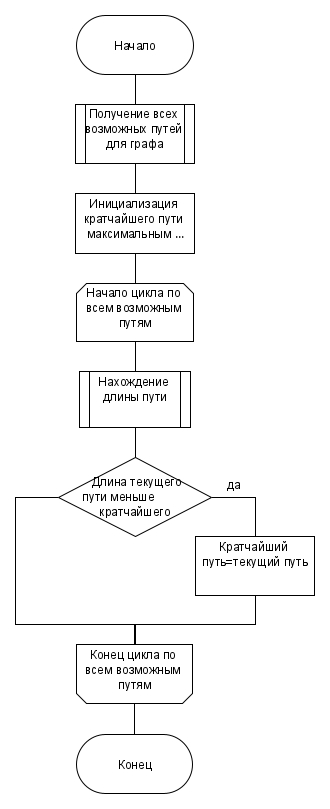
\includegraphics[width=0.5\linewidth]{src/bf}
	\caption{Алгоритм полного перебора}
	\label{fig:bf}
\end{figure}
\begin{figure}[H]
	\centering
	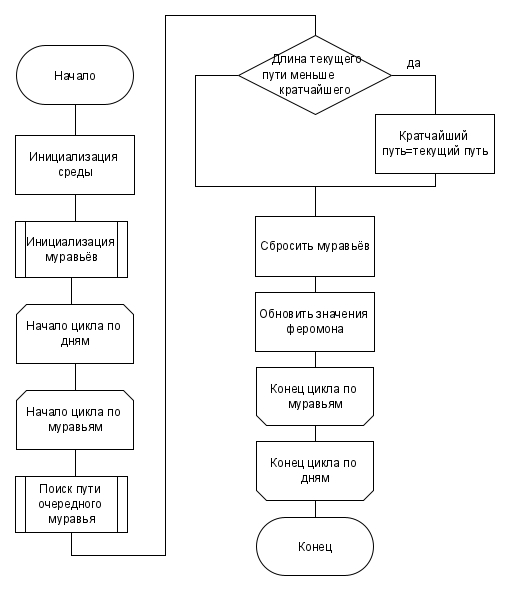
\includegraphics[width=0.7\linewidth]{src/ant}
	\caption{Муравьиный алгоритм}
	\label{fig:ant}
\end{figure}

\section{Параметризация и трудоёмкость муравьиного алгоритма}
\label{sec:parametrisation}
На эффективность алгоритма влияют параметры: коэффициенты жадности и стадности, коэффициент испарения феромона, количество поколений. 
\par Для получения их оптимальной комбинации производится параметризация -- полный перебор в цикле этих параметров. Для каждой их комбинации производится 2 поиска маршрута для каждой из 2-х карт, из этих двух маршрутов выбирается по минимальному и она  записывается в файл вместе с разностями длин полученных маршрутов и эталонного.
\par Трудоёмкость его $O(t_{max}*max(m,n^2))$.

\section{Вывод}
\label{sec:design_conclusion}
В данном разделе были рассмотрены схемы алгоритма полного перебора и муравьиного алгоритма, описана параметризация последнего.